% !TEX root = ../../main.tex

\subsection{Simulation Setup and Evaluation Metrics}

This section defines the simulation setting used to evaluate the baseline OFDM-LMMSE system, the baseline OTFS system, and the proposed OTFS-IM schemes. The purpose is to make the numerical results in the following sections reproducible and rate-aware. Since OTFS-IM changes both the signal structure and the number of information bits carried by each delay-Doppler block, the evaluation cannot rely only on BER curves. The simulation setup must also specify the spectral efficiency of each configuration and the error components associated with index modulation.

\subsubsection{Simulation Parameters}

All schemes are evaluated over the same delay-Doppler channel realization model and the same \(E_b/N_0\) range. The OTFS frame consists of \(N=10\) Doppler bins and \(M=12\) delay bins, resulting in \(NM=120\) resource elements per frame. The baseline OTFS and OFDM systems use 4-QAM modulation over all resource elements. The OTFS-IM system also uses 4-QAM on active positions, while additional information is conveyed by the activation pattern inside each IM block.

The channel is modeled as a discrete time-varying multipath channel with three propagation paths. The implemented delay taps are \([0,1,2]\), while the Doppler taps are randomly generated integer values in the simulated Doppler grid. Therefore, the simulation represents a Doppler-spread doubly selective channel rather than a channel tied to a specific physical velocity value. This choice is consistent with the purpose of the thesis: evaluating OTFS and OTFS-IM under delay-Doppler channel variations associated with high-mobility communication scenarios, without claiming a particular vehicular speed.

Table~\ref{tab:chapter5_simulation_parameters} summarizes the main simulation parameters used in the numerical evaluation.

\begin{table}[H]
    \centering
    \caption{Main simulation parameters}
    \label{tab:chapter5_simulation_parameters}
    \begin{tabularx}{\linewidth}{>{\RaggedRight\arraybackslash}p{4.4cm}
                                  >{\RaggedRight\arraybackslash}p{4.2cm}
                                  >{\RaggedRight\arraybackslash}X}
        \toprule
        Parameter & Value & Role in the simulation \\
        \midrule
        Doppler bins, \(N\) & 10 & Number of Doppler-domain grid points per OTFS frame \\
        \midrule
        Delay bins, \(M\) & 12 & Number of delay-domain grid points per OTFS frame \\
        \midrule
        Total resource elements & \(NM=120\) & Number of transmitted grid symbols per frame \\
        \midrule
        Baseline modulation & 4-QAM & Modulation used by OFDM-LMMSE and baseline OTFS \\
        \midrule
        Active-symbol modulation in OTFS-IM & 4-QAM & Modulation used on active IM positions \\
        \midrule
        Channel model & 3-tap delay-Doppler channel & Common channel model for OFDM, OTFS, and OTFS-IM \\
        \midrule
        Delay taps & \([0,1,2]\) & Discrete multipath delay positions \\
        \midrule
        Doppler taps & Random integer Doppler taps & Time variation and Doppler-spread behavior \\
        \midrule
        \(E_b/N_0\) range & \(0:5:20\) dB & SNR range used for BER curves \\
        \midrule
        OFDM-LMMSE frames & 1000 & Number of simulated OFDM frames per SNR point \\
        \midrule
        OTFS and OTFS-IM frames & 1000 & Number of simulated OTFS/OTFS-IM frames per SNR point \\
        \midrule
        Random-pattern diagnostic & 5 tables, 100 frames/table & Validation baseline for pattern-selection methods \\
        \bottomrule
    \end{tabularx}
\end{table}

The tested OTFS-IM configurations are selected to cover both equal-rate and reliability-oriented cases. Equal-rate configurations have the same spectral efficiency as the baseline OTFS system, while lower-rate configurations are included to show how reducing the number of transmitted bits per resource element can affect BER. For an IM block with \(n\) positions and \(k\) active positions, the number of index bits per block is
\begin{equation}
    b_1 = \left\lfloor \log_2 \binom{n}{k} \right\rfloor,
    \label{eq:chapter5_index_bits}
\end{equation}
and the number of active-symbol bits per block is
\begin{equation}
    b_2 = k \log_2 M_{\mathrm{QAM}}.
    \label{eq:chapter5_symbol_bits}
\end{equation}
Since 4-QAM is used in this thesis, \(\log_2 M_{\mathrm{QAM}}=2\). The spectral efficiency of the OTFS-IM mapping is then
\begin{equation}
    \eta_{\mathrm{IM}} = \frac{b_1+b_2}{n}.
    \label{eq:chapter5_im_spectral_efficiency}
\end{equation}

\begin{figure}[H]
    \centering
    \resizebox{0.98\linewidth}{!}{%
    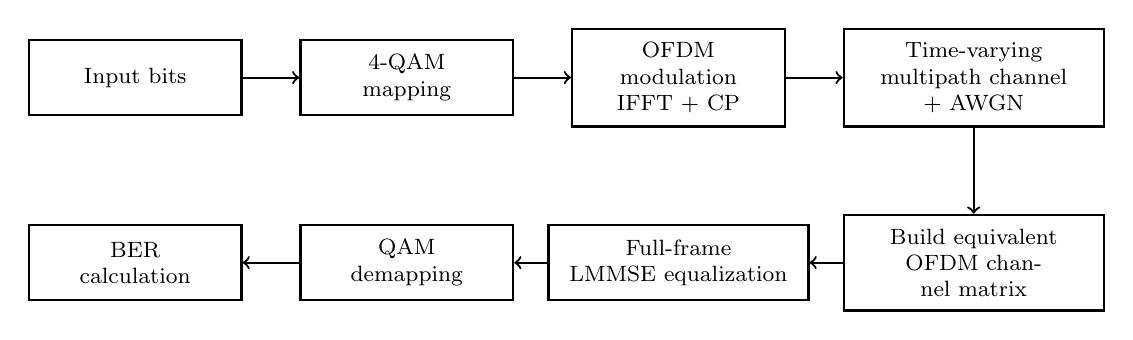
\begin{tikzpicture}[
        block/.style={
            rectangle,
            draw,
            thick,
            align=center,
            text width=2.35cm,
            minimum height=0.95cm,
            font=\footnotesize,
            inner sep=5pt
        },
        wideblock/.style={
            rectangle,
            draw,
            thick,
            align=center,
            text width=2.95cm,
            minimum height=0.95cm,
            font=\footnotesize,
            inner sep=5pt
        },
        arrow/.style={->, thick}
    ]
        \node[block] (bits) at (0,0) {Input bits};
        \node[block] (qam) at (3.45,0) {4-QAM\\mapping};
        \node[block] (ofdm) at (6.90,0) {OFDM\\modulation\\IFFT + CP};
        \node[wideblock] (chan) at (10.65,0) {Time-varying\\multipath channel\\+ AWGN};
        \node[wideblock] (hmat) at (10.65,-2.35) {Build equivalent\\OFDM channel matrix};
        \node[wideblock] (lmmse) at (6.90,-2.35) {Full-frame\\LMMSE equalization};
        \node[block] (demap) at (3.45,-2.35) {QAM\\demapping};
        \node[block] (ber) at (0,-2.35) {BER\\calculation};

        \draw[arrow] (bits.east) -- (qam.west);
        \draw[arrow] (qam.east) -- (ofdm.west);
        \draw[arrow] (ofdm.east) -- (chan.west);
        \draw[arrow] (chan.south) -- (hmat.north);
        \draw[arrow] (hmat.west) -- (lmmse.east);
        \draw[arrow] (lmmse.west) -- (demap.east);
        \draw[arrow] (demap.west) -- (ber.east);
    \end{tikzpicture}
    }
    \caption{OFDM-LMMSE baseline simulation flow}
    \label{fig:chapter5_ofdm_lmmse_flow}
\end{figure}

The OFDM-LMMSE flow in Fig.~\ref{fig:chapter5_ofdm_lmmse_flow} clarifies how the conventional multicarrier baseline is generated in the simulation. The receiver does not simply apply one-tap equalization; instead, it uses a full-frame LMMSE equalizer with channel knowledge. This makes the OFDM reference a stronger baseline for comparison with the delay-Doppler OTFS and OTFS-IM receivers.

Table~\ref{tab:chapter5_im_configurations} lists all simulated OTFS-IM configurations. The baseline OTFS and OFDM-LMMSE systems both have spectral efficiency \(2.00\) bits/symbol under 4-QAM transmission.

\begin{table}[H]
    \centering
    \caption{Simulated OTFS-IM configurations}
    \label{tab:chapter5_im_configurations}
    \begin{tabularx}{\linewidth}{>{\centering\arraybackslash}p{2.4cm}
                                  >{\centering\arraybackslash}p{1.4cm}
                                  >{\centering\arraybackslash}p{1.4cm}
                                  >{\centering\arraybackslash}p{1.4cm}
                                  >{\centering\arraybackslash}p{1.4cm}
                                  >{\centering\arraybackslash}p{2.4cm}
                                  >{\RaggedRight\arraybackslash}X}
        \toprule
        Configuration & \(n\) & \(k\) & \(b_1\) & \(b_2\) & \(\eta_{\mathrm{IM}}\) & Interpretation \\
        \midrule
        \(4\)-\(2\) & 4 & 2 & 2 & 4 & 1.50 & Lower-SE reliability-oriented case \\
        \midrule
        \(4\)-\(3\) & 4 & 3 & 2 & 6 & 2.00 & Equal-SE case \\
        \midrule
        \(5\)-\(3\) & 5 & 3 & 3 & 6 & 1.80 & Main pattern-selection validation case \\
        \midrule
        \(5\)-\(4\) & 5 & 4 & 2 & 8 & 2.00 & Equal-SE case \\
        \midrule
        \(6\)-\(3\) & 6 & 3 & 4 & 6 & 1.67 & Lower-SE reliability-oriented case \\
        \midrule
        \(6\)-\(4\) & 6 & 4 & 3 & 8 & 1.83 & Supplementary trade-off case \\
        \midrule
        \(6\)-\(5\) & 6 & 5 & 2 & 10 & 2.00 & Main larger-block equal-SE case \\
        \bottomrule
    \end{tabularx}
\end{table}

\subsubsection{Compared Schemes and Evaluation Metrics}

Four main schemes are compared in Chapter 5. The first one is OFDM-LMMSE, which is used as the conventional multicarrier reference. In the implementation, OFDM symbols are transmitted over the same time-varying channel as OTFS, and the receiver applies a full-frame LMMSE equalizer with perfect channel knowledge. Therefore, the OFDM curve should be understood as an equalized OFDM baseline, not as an unequalized OFDM receiver. This makes the comparison more meaningful because OTFS and OTFS-IM are not compared against an intentionally weak OFDM receiver.

The second scheme is the baseline OTFS system developed in Chapter 3. It uses full-grid 4-QAM mapping in the delay-Doppler domain and serves as the direct reference for evaluating whether OTFS-IM provides a useful improvement. The third scheme is OHD OTFS-IM, where the activation-pattern table is selected according to the optimized Hamming-distance criterion. The fourth scheme is B-OHD OTFS-IM, where the pattern-selection process additionally considers balance-related criteria such as carrier usage and closest-pair behavior. In configurations where OHD and B-OHD select effectively the same pattern set, their BER curves can overlap. This is not a simulation error; it means that the additional B-OHD criteria do not change the selected table for that specific \((n,k)\) setting.

Random pattern tables are also simulated as a diagnostic baseline. They are not treated as a proposed transmission method. Their role is to test whether deterministic pattern selection actually gives a meaningful advantage over arbitrary valid pattern choices. If a random table performs close to OHD or B-OHD in some SNR region, the result should be interpreted as evidence that pattern geometry alone is not always sufficient to determine the final BER.

The primary performance metric is the total bit error rate,
\begin{equation}
    \mathrm{BER} = \frac{N_{\mathrm{err}}}{N_{\mathrm{bits}}},
    \label{eq:chapter5_ber_definition}
\end{equation}
where \(N_{\mathrm{err}}\) is the number of incorrectly detected bits and \(N_{\mathrm{bits}}\) is the total number of transmitted information bits. For OTFS and OFDM, this BER directly measures the reliability of QAM symbol detection. For OTFS-IM, the total BER contains both index-bit errors and symbol-bit errors.

To explain the OTFS-IM behavior more clearly, the total BER is decomposed into index BER and symbol BER. Index BER measures the reliability of recovering the activation-pattern bits \(b_1\), while symbol BER measures the reliability of recovering the QAM bits \(b_2\) placed on active positions. In addition, the pattern error rate is reported as
\begin{equation}
    \mathrm{PER} = \frac{N_{\mathrm{wrong\ pattern}}}{N_{\mathrm{IM\ blocks}}},
    \label{eq:chapter5_pattern_error_rate}
\end{equation}
where \(N_{\mathrm{wrong\ pattern}}\) is the number of IM blocks in which the selected activation pattern is detected incorrectly. This metric is important because a wrong pattern decision can cause both index errors and symbol-placement errors.

Finally, spectral efficiency is used to distinguish equal-rate gains from rate-reliability trade-offs. A BER reduction is strongest when it is obtained at \(\eta_{\mathrm{IM}}=2.00\) bits/symbol, because this matches the spectral efficiency of the baseline OTFS system. If a configuration has lower BER but also lower spectral efficiency, the result is still useful, but it should be interpreted as a reliability-oriented trade-off rather than an unconditional improvement. For this reason, the final part of Chapter 5 presents both a configuration-level BER summary and a BER-SE trade-off plot across all simulated configurations.
